% ---
% titre: Calculer avec des nombres relatifs
% theme: NO
% chapitre: Nombres relatifs
% sous_chapitre: Addition et soustraction
% niveau: [9e,10e,11e]
% type: EX
% tags: [c-addition,c-division,c-multiplication,c-operations,c-soustraction,c-nombres-relatifs, f-individuel,f-maison,f-station,p-entrainement,p-remediation]
% difficulte: 2
% source: latex
% ---

\header{Additions et soustractions de nombres relatifs}

{\small
\bigskip
\def\arraystretch{1.7}
\begin{tabularx}{\linewidth}{*{4}{X}}
\textbf{A.} & \textbf{B.} & \textbf{C.} & \textbf{D.} \\
$(+11)+(-6)= \sol{\dotfill}{+5}$   & $(-8)+(+13)= \sol{\dotfill}{+5}$   & $(+13)+(-18)= \sol{\dotfill}{-5}$ & $(-6)-(+12)= \sol{\dotfill}{-18}$   \\
$(+9)-(+15)= \sol{\dotfill}{-6}$  & $(+17)+(-22)= \sol{\dotfill}{-5}$ & $(-13)+(-15)= \sol{\dotfill}{-28}$ & $(+11)-(-11)= \sol{\dotfill}{+22}$   \\
$(+7)+(+14)= \sol{\dotfill}{+21}$  & $(-20)-(-18)= \sol{\dotfill}{-2}$ & $(+12)+(-12)= \sol{\dotfill}{0}$   & $(+27)-(+17)= \sol{\dotfill}{+10}$ \\
$(-27)-(+15)= \sol{\dotfill}{-42}$ & $(+12)+(+16)= \sol{\dotfill}{+28}$  & $(-15)+(-11)= \sol{\dotfill}{-26}$  & $(-17)+(-10)= \sol{\dotfill}{-27}$  \\
$(+18)-(-10)= \sol{\dotfill}{+28}$  & $(+13)-(-12)= \sol{\dotfill}{+25}$  & $(+17)+(-8)= \sol{\dotfill}{+9}$  & $(-18)-(-20)= \sol{\dotfill}{+2}$ \\
$(+17)+(-11)= \sol{\dotfill}{+6}$  & $(+15)-(-4)= \sol{\dotfill}{+19}$  & $(-8)-(-17)= \sol{\dotfill}{+9}$  & $(+23)-(+21)= \sol{\dotfill}{+2}$ \\
\end{tabularx}
}

\header{Simplification d'écriture et somme algébrique}

{\bfseries\color{themeColor}Exercice 1.} \quad$(+9) + (-6) - (+8) + (-3) + (+11) - (-7) =$

\sol{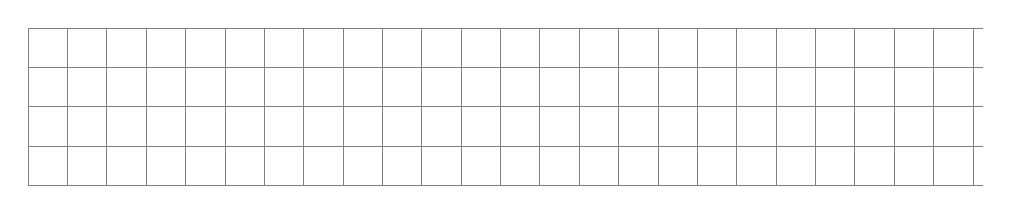
\begin{tikzpicture}\draw[step=0.5cm, gray, very thin] (0,0) grid (\textwidth,2);\end{tikzpicture}}{
$(+9) + (-6) - (+8) + (-3) + (+11) - (-7) = +9 -6 -8 -3 +11 +7 = +27-17 = 10$}

{\bfseries\color{themeColor}Exercice 2.} \quad$(-14) + (+5) - (-7) + (+9) - (+11) + (-6) =$

\sol{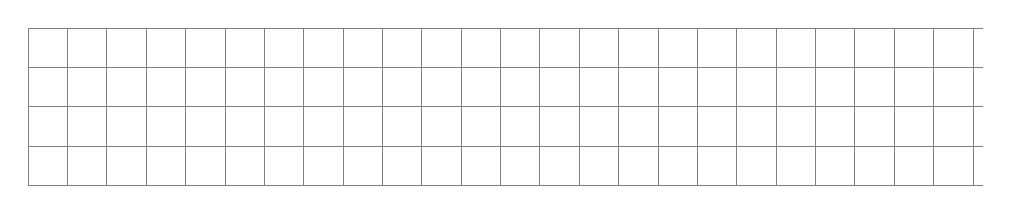
\begin{tikzpicture}\draw[step=0.5cm, gray, very thin] (0,0) grid (\textwidth,2);\end{tikzpicture}}{
$(-14) + (+5) - (-7) + (+9) - (+11) + (-6) = -14 +5 +7 +9 -11 -6 = +21-31 = -10$}

{\bfseries\color{themeColor}Exercice 3.} \quad$(-28) - (+15) + (-19) - (-28) + (+33)=$

\sol{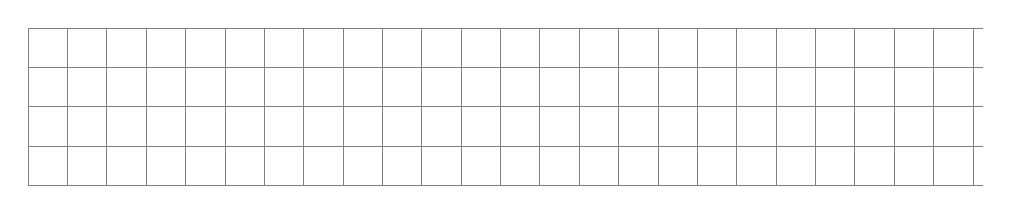
\begin{tikzpicture}\draw[step=0.5cm, gray, very thin] (0,0) grid (\textwidth,2);\end{tikzpicture}}{
$(-28) - (+15) + (-19) - (-28) + (+33) = -28 -15 -19 +28 +33 = +61-62 = -1$}

{\bfseries\color{themeColor}Exercice 4.} \quad$(-18) + (-12) - (-9) - (-6) + (+14) + (+10) =$

\sol{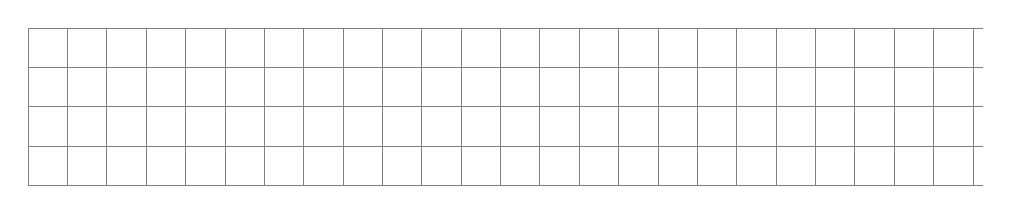
\begin{tikzpicture}\draw[step=0.5cm, gray, very thin] (0,0) grid (\textwidth,2);\end{tikzpicture}}{
$(-18) + (-12) - (-9) - (-6) + (+14) + (+10) = -18 -12 +9 +6 +14 +10 = +39-30 = 9$}

{\bfseries\color{themeColor}Exercice 5.} \quad$(+20) - (-15) + (-25) + (-18) + (+22) - (-30) =$

\sol{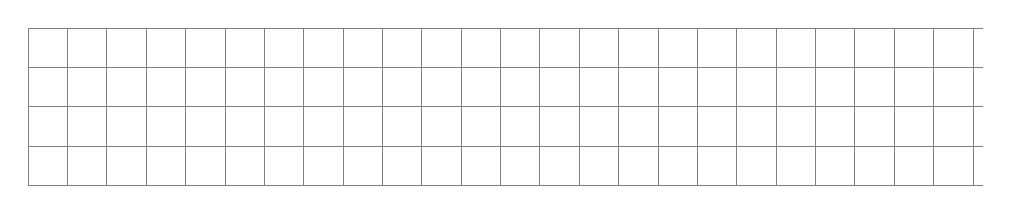
\begin{tikzpicture}\draw[step=0.5cm, gray, very thin] (0,0) grid (\textwidth,2);\end{tikzpicture}}{
$(+20) - (-15) + (-25) + (-18) + (+22) - (-30) = +20 +15 -25 -18 +22 +30 = +87-43 = 44$}

{\bfseries\color{themeColor}Exercice 6.} \quad$(-11) + (+9) - (-13) + (+16) - (-5) =$

\sol{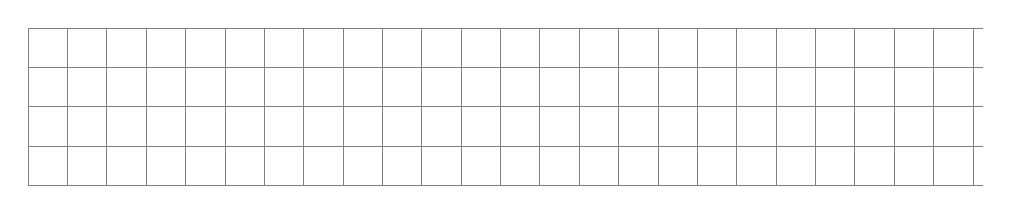
\begin{tikzpicture}\draw[step=0.5cm, gray, very thin] (0,0) grid (\textwidth,2);\end{tikzpicture}}{
$(-11) + (+9) - (-13) + (+16) - (-5) = -11 +9 +13 +16 +5 = +43-11 = 32$}

{\bfseries\color{themeColor}Exercice 7.} \quad$(-17) + (+8) - (+10) + (-14) - (-19) + (+21) =$

\sol{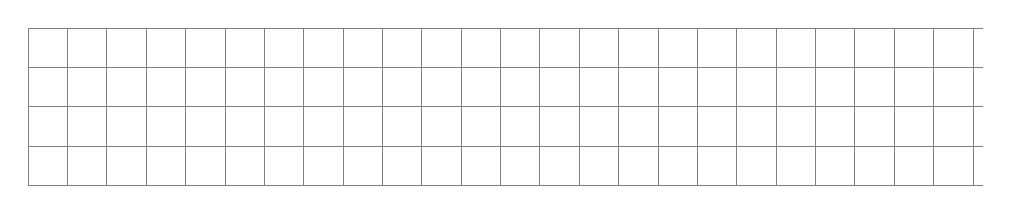
\begin{tikzpicture}\draw[step=0.5cm, gray, very thin] (0,0) grid (\textwidth,2);\end{tikzpicture}}{
$(-17) + (+8) - (+10) + (-14) - (-19) + (+21) = -17 +8 -10 -14 +19 +21 = +48-41 = 7$}

{\bfseries\color{themeColor}Exercice 8.} \quad$(-9) + (-12) - (+7) + (+5) - (-3) + (+16) =$

\sol{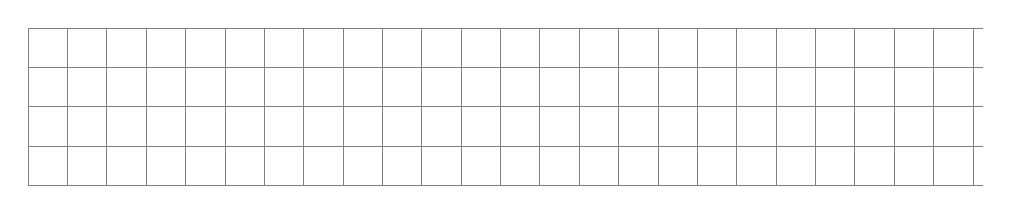
\begin{tikzpicture}\draw[step=0.5cm, gray, very thin] (0,0) grid (\textwidth,2);\end{tikzpicture}}{
$(-9) + (-12) - (+7) + (+5) - (-3) + (+16) = -9 -12 -7 +5 +3 +16 = +24-28 = -4$}

{\bfseries\color{themeColor}Exercice 9.} \quad$(-19) + (-22) - (-14) - (+17) + (+38) =$

\sol{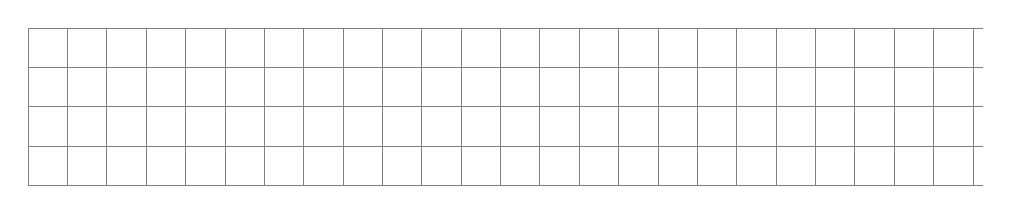
\begin{tikzpicture}\draw[step=0.5cm, gray, very thin] (0,0) grid (\textwidth,2);\end{tikzpicture}}{
$(-19) + (-22) - (-14) - (+17) + (+38) = -19 -22 +14 -17 +38 = +52-58 = -6$}

{\bfseries\color{themeColor}Exercice 10.} \quad$(+13) - (+9) - (-11) + (-6) + (+15) - (-8) =$

\sol{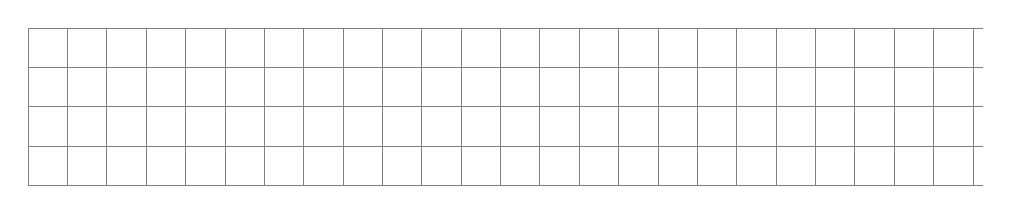
\begin{tikzpicture}\draw[step=0.5cm, gray, very thin] (0,0) grid (\textwidth,2);\end{tikzpicture}}{
$(+13) - (+9) - (-11) + (-6) + (+15) - (-8) = +13 -9 +11 -6 +15 +8 = +47-15 = 32$}


\vfill
\header{Multiplications et divisions de nombres relatifs}

{\small
\bigskip
\def\arraystretch{1.7}
\begin{tabularx}{\linewidth}{*{4}{X}}
\textbf{A.} & \textbf{B.} & \textbf{C.} & \textbf{D.} \\
$(+7)\cdot(-4)= \dotfill$    & $(-56):(+8)= \dotfill$  & $(+63):(-9)= \dotfill$      & $(+32):(+8)= \dotfill$      \\
$(+9)\cdot(+8)= \dotfill$   & $(-18):(-9)= \dotfill$  & $(-12)\cdot(-10)= \dotfill$ & $(+6)\cdot(-7)= \dotfill$   \\
$(+7)\cdot(+9)= \dotfill$   & $(+80):(-10)= \dotfill$ & $(+8)\cdot(-8)= \dotfill$   & $(-54):(+6)= \dotfill$      \\
$(+36):(-6)= \dotfill$       & $(-84):(+12)= \dotfill$ & $(-15):(-5)= \dotfill$      & $(+13)\cdot(-9)= \dotfill$ \\
$(+108):(-12)= \dotfill$      & $(+9)\cdot(-5)= \dotfill$ & $(+30):(-6)= \dotfill$    & $(-56):(-8)= \dotfill$      \\
$(+64):(-8)= \dotfill$       & $(+36):(+9)= \dotfill$  & $(-7)\cdot(-8)= \dotfill$   & $(+12):(-12)= \dotfill$     \\
\end{tabularx}
}

\newpage
\header{C'est en forgeant que l'on devient forgeron !}

{\small
\bigskip
\def\arraystretch{1.2}
\begin{tabularx}{\linewidth}{*{4}{X}}
\textbf{A.} & \textbf{B.} & \textbf{C.} & \textbf{D.} \\
$(+17)-(-19)= \dotfill$ & $(-14)\cdot(+9)= \dotfill$ & $(-11)+(+8)= \dotfill$ & $(-9)+(+25)= \dotfill$ \\
$(+27)+(-38)= \dotfill$ & $(-18)\cdot(-6)= \dotfill$ & $(+120)+(-40)= \dotfill$ & $(+45)+(-18)= \dotfill$ \\
$(+16)\cdot(-7)= \dotfill$ & $(+210):(-7)= \dotfill$ & $(+160)-(-95)= \dotfill$ & $(+38)-(-52)= \dotfill$ \\
$(-135):(-5)= \dotfill$ & $(-27):(+9)= \dotfill$ & $(+29)+(-6)= \dotfill$ & $(-38)-(-24)= \dotfill$ \\
$(+29)+(-46)= \dotfill$ & $(+63)+(-34)= \dotfill$ & $(-15)\cdot(+45)= \dotfill$ & $(-9)\cdot(+6)= \dotfill$ \\
$(+18)\cdot(-5)= \dotfill$ & $(-38)+(+61)= \dotfill$ & $(+360)+(-15)= \dotfill$ & $(-11)\cdot(-9)= \dotfill$ \\
$(+48)-(+19)= \dotfill$ & $(-27)-(+58)= \dotfill$ & $(+150)+(-90)= \dotfill$ & $(-108):(-9)= \dotfill$ \\
$(-95):(+5)= \dotfill$ & $(+43)-(+28)= \dotfill$ & $(-54):(-18)= \dotfill$ & $(+63):(-7)= \dotfill$ \\
\end{tabularx}

\bigskip
\begin{tabularx}{\linewidth}{*{4}{X}}
\textbf{E.} & \textbf{F.} & \textbf{G.} & \textbf{H.} \\
$(+58)-(-23)= \dotfill$ & $(-16)\cdot(+9)= \dotfill$ & $(-14)+(+21)= \dotfill$ & $(-19)+(-16)= \dotfill$ \\
$(+31)+(-45)= \dotfill$ & $(-12)\cdot(-9)= \dotfill$ & $(-21)+(+37)= \dotfill$ & $(-19)+(+29)= \dotfill$ \\
$(-13)\cdot(+6)= \dotfill$ & $(+170):(-5)= \dotfill$ & $(+34)+(+29)= \dotfill$ & $(-120)+(+95)= \dotfill$ \\
$(-60):(-20)= \dotfill$ & $(-72):(+8)= \dotfill$ & $(-28)+(-17)= \dotfill$ & $(-38)+(-19)= \dotfill$ \\
$(+33)+(-51)= \dotfill$ & $(+19)+(-14)= \dotfill$ & $(+27)+(+31)= \dotfill$ & $(+42)+(+37)= \dotfill$ \\
$(+12)\cdot(-6)= \dotfill$ & $(-29)+(+53)= \dotfill$ & $(-34)+(-41)= \dotfill$ & $(-52)+(+95)= \dotfill$ \\
$(+41)-(+19)= \dotfill$ & $(-38)-(-64)= \dotfill$ & $(+140)+(-95)= \dotfill$ & $(-135)+(+62)= \dotfill$ \\
$(+90):(-2)= \dotfill$ & $(+38)-(+21)= \dotfill$ & $(-144):(+12)= \dotfill$ & $(+49)+(+36)= \dotfill$ \\
\end{tabularx}

\bigskip
\begin{tabularx}{\linewidth}{*{4}{X}}
\textbf{I.} & \textbf{J.} & \textbf{K.} & \textbf{L.} \\
$(+17)-(-14)= \dotfill$ & $(-9)\cdot(-13)= \dotfill$ & $(-23)+(-16)= \dotfill$ & $(-58)+(-34)= \dotfill$ \\
$(+19)-(-64)= \dotfill$ & $(-16)\cdot(-5)= \dotfill$ & $(+34)+(-51)= \dotfill$ & $(-31)+(+72)= \dotfill$ \\
$(-17)-(-29)= \dotfill$ & $(-11)\cdot(-11)= \dotfill$ & $(-39)+(+14)= \dotfill$ & $(-135)+(+118)= \dotfill$ \\
$(+37)-(+18)= \dotfill$ & $(-9)\cdot(+14)= \dotfill$ & $(+67)+(+45)= \dotfill$ & $(-128)+(+29)= \dotfill$ \\
$(+38)-(-21)= \dotfill$ & $(+160)\cdot(-5)= \dotfill$ & $(-54)+(-27)= \dotfill$ & $(+83)+(+31)= \dotfill$ \\
$(+34)-(+16)= \dotfill$ & $(-11)\cdot(-9)= \dotfill$ & $(+57)+(+42)= \dotfill$ & $(-73)+(+141)= \dotfill$ \\
$(-51)-(-18)= \dotfill$ & $(+21)\cdot(-6)= \dotfill$ & $(-46)+(+59)= \dotfill$ & $(-162)+(+58)= \dotfill$ \\
$(-49)-(-27)= \dotfill$ & $(-14)\cdot(-8)= \dotfill$ & $(+165)+(-105)= \dotfill$ & $(+81)+(+46)= \dotfill$ \\
\end{tabularx}

\bigskip
\begin{tabularx}{\linewidth}{*{4}{X}}
\textbf{M.} & \textbf{N.} & \textbf{O.} & \textbf{P.} \\
$(-19)+(-48)= \dotfill$ & $(-24)+(+53)= \dotfill$ & $(-14)-(+21)= \dotfill$ & $(+46)-(-37)= \dotfill$ \\
$(+110)\cdot(-4)= \dotfill$ & $(+38)+(+64)= \dotfill$ & $(-1)\cdot(+95)= \dotfill$ & $(-54)+(+28)= \dotfill$ \\
$(+3)\cdot(-58)= \dotfill$ & $(-67)-(-79)= \dotfill$ & $(+15)+(-72)= \dotfill$ & $(-45):(-5)= \dotfill$ \\
$(-83):(+10)= \dotfill$ & $(-58)-(-19)= \dotfill$ & $(-96):(-8)= \dotfill$ & $(-142)+(-9)= \dotfill$ \\
$(+23):(-0{,}5)= \dotfill$ & $(+15)\cdot(+7)= \dotfill$ & $(-31)-(+31)= \dotfill$ & $(-64)\cdot(-15)= \dotfill$ \\
$(-73)+(+39)= \dotfill$ & $(-84)\cdot(+25)= \dotfill$ & $(-84):(+4)= \dotfill$ & $(+14)\cdot(+45)= \dotfill$ \\
$(-28)-(+54)= \dotfill$ & $(-63):(-2)= \dotfill$ & $(+118)+(-142)= \dotfill$ & $(+86)-(-14)= \dotfill$ \\
$(-17)-(-74)= \dotfill$ & $(+186):(-93)= \dotfill$ & $(-16)\cdot(-7)= \dotfill$ & $(-138)+(-16)= \dotfill$ \\
\end{tabularx}}